\documentclass[pdflatex,sn-nature]{sn-jnl}% Style for submissions to Nature Portfolio journals

\usepackage{graphicx}%
\usepackage{multirow}%
\usepackage{amsmath,amssymb,amsfonts}%
\usepackage{amsthm}%
\usepackage{mathrsfs}%
\usepackage[title]{appendix}%
\usepackage{xcolor}%
\usepackage{textcomp}%
\usepackage{manyfoot}%
\usepackage{booktabs}%
\usepackage{threeparttable}
\usepackage{siunitx}
\usepackage{caption}
\usepackage{algorithm}%
\usepackage{algorithmicx}%
\usepackage{algpseudocode}%
\usepackage{listings}%
\usepackage{siunitx}

%%%%
\theoremstyle{thmstyleone}%
\newtheorem{theorem}{Theorem}%  meant for continuous numbers
%%\newtheorem{theorem}{Theorem}[section]% meant for sectionwise numbers
%% optional argument [theorem] produces theorem numbering sequence instead of independent numbers for Proposition
\newtheorem{proposition}[theorem]{Proposition}% 
%%\newtheorem{proposition}{Proposition}% to get separate numbers for theorem and proposition etc.
\newcommand{\norm}[1]{\left\|#1\right\|}
\theoremstyle{thmstyletwo}%
\newtheorem{example}{Example}%
\newtheorem{remark}{Remark}%

\theoremstyle{thmstylethree}%
\newtheorem{definition}{Definition}%

\raggedbottom
%%\unnumbered% uncomment this for unnumbered level heads

\begin{document}

\title[Integrating Fundamental Knowledge and Sensor Data: Physics-Informed Neural Networks for Smart Agricultural Water Management]{Integrating Fundamental Knowledge and Sensor Data: Physics-Informed Neural Networks for Smart Agricultural Water Management}






\author*[1]{\fnm{Gregory} \sur{Conde}}\email{gregory.condemen@ufl.edu}

\author[1]{\fnm{Sandra M.} \sur{Guzmán}}\email{sandra.guzmangut@ufl.edu}

\author[2]{\fnm{Jorge I.} \sur{Poveda}}\email{jipoveda@ucsd.edu}

\author[3]{\fnm{Flavia T.} \sur{Zambon}}\email{f.zambon@ufl.edu}


\affil*[1]{\orgdiv{Agricultural and Biological Engineering, Indian River Research and Education Center}, \orgname{University of Florida}, \orgaddress{\city{Fort Pierce}, \postcode{34945}, \state{Florida}, \country{USA}}}

\affil[2]{\orgdiv{Department of Electrical and Computer Engineering}, \orgname{University of California}, \orgaddress{\city{San Diego}, \postcode{92093}, \state{California}, \country{USA}}}

\affil[3]{\orgdiv{Institute of Food and Agricultural Sciences, Indian River Research and Education Center}, \orgname{University of Florida}, \orgaddress{\city{Fort Pierce}, \postcode{34945}, \state{Florida}, \country{USA}}}



%%==================================%%
%% Sample for unstructured abstract %%
%%==================================%%
\abstract{Agriculture accounts for 70\% of global freshwater use, yet irrigation inefficiency threatens food security as water scarcity intensifies. Accurate soil moisture prediction for decision-making is crucial for sustainable water management in horticultural systems; however, traditional approaches face an unresolved challenge: analytical models oversimplify the complex dynamics of soil-water-plant interactions, while purely data-driven methods lack the physical consistency required for reliable control decisions. Here, we present a physics-informed neural network (PINN) that addresses this by embedding the principles of Richards' equation into a deep learning architecture, enabling control-oriented modeling and decision-making in irrigation systems. The PINN discretizes Richards' equation spatially, modeling flow through constrained neural branches that yield physically consistent ordinary differential equations at sensor depths. Trained alongside its numerical solution to ensure stability, the model predicts soil moisture in citrus fields with a 1.25\% volumetric water content RMSE over 3-day forecasts and infers depth-specific crop water uptake, a key management variable that has previously been difficult to measure. This approach enables predictive control for precision irrigation in horticultural production, offering a pathway to sustainable consumption and production under increasingly variable climate conditions.}

%\keywords{Water, Smart Irrigation, Physics Informed Neural Networks, PINN, Modeling, Soil Moisture, Richards' equation}





\maketitle

Agriculture consumes 70\% of global freshwater\cite{scanlon2023}, yet irrigation efficiency remains below 50\% in many regions\cite{Mehta2024}, resulting in the wasteful use of a resource essential for food security. Smart irrigation systems, which utilize sensors and algorithms to optimize water delivery, offer a solution; however, their widespread adoption faces a critical technical barrier: current approaches cannot integrate real-time soil moisture data, weather forecasts, and plant water demands into models capable of predictive control. The result is irrigation management that remains largely reactive rather than anticipatory, missing opportunities to reduce water use while maintaining crop productivity.

%--- Move 2: Practical & Scientific Gaps --------------------------------------

The technical gap is well-defined. Smart irrigation algorithms are necessary to pinpoint the precise locations where water should be supplied as plant root systems develop. During germination, water must reach the topsoil layers where seeds are planted; as crops develop, deeper soil layers become critical. Although studies provide general depth guidelines for certain crop types \cite{ASABE2021}, the ability to precisely locate where plants require water based on real-time crop data remains elusive. Algorithms must account for how irrigation, rainfall, plant water uptake, and environmental conditions collectively influence soil water content (SWC) across depths, ideally integrating weather forecasts to predict soil moisture response to upcoming irrigation events. Current approaches fall short: one method uses potential evapotranspiration and crop coefficients to calculate water requirements \cite{Volk2024}; another irrigates based on sensor thresholds between field capacity and maximum allowable depletion \cite{zhang2021}. Neither incorporates current soil moisture, anticipated dynamics, predicted rainfall, and projected crop demands into a unified predictive framework suitable for optimization algorithms.
The modeling challenge is formidable. Capturing plant-soil-water interactions at multiple depths requires confronting: (i) the dynamic nature of plant growth and water uptake, which varies with crop type, phenology, and environmental conditions; (ii) the nonlinearity of Richards' equation governing vertical water movement in unsaturated soils, which demands complex numerical methods \cite{Celia1990}; (iii) the empirical constitutive models (e.g., Gardner, van Genuchten, Brooks–Corey) that represent gravitational and capillary forces in Richards' equation, requiring labor-intensive parameter calibration and lacking universal applicability across soil types \cite{Pan2019}; and (iv) the coarse spatial and temporal resolution of available data, which forces discretizations that can violate numerical stability criteria \cite{Celia1990,leveque2007}. Traditional analytical models are computationally expensive and require soil hydraulic parameters that vary unpredictably in heterogeneous fields. Purely data-driven machine learning models can predict soil moisture, but they produce "black box" outputs that lack the physical consistency and stability guarantees necessary for model predictive control.
%--- Move 3: Opportunity & Approach -------------------------------------------

Here, we resolve this dichotomy through physics-informed neural networks (PINNs), a technique that unifies neural network function approximation, machine learning tools, established soil-water dynamics theory, and plant biophysics into models suitable for smart irrigation management. Originally developed to reduce computational costs when solving partial differential equations (PDEs) \cite{Cuomo2022}, PINNs overcome the limitations of purely data-driven approaches (vast data requirements and lack of physical consistency) and analytical models (computational expense and system-specific governing equations). 


%--- Move 4: Prior Art & Positioning
Recent applications demonstrate the potential of PINNs for control-oriented modeling in high-uncertainty systems, such as automated vehicles and quantum systems \cite{Li2024, Zhang2025}. In soil sciences, PINNs have been explored as alternatives to numerical solutions of Richards' equation \cite{Bandai2022}, for handling sparse data in unsaturated infiltration modeling \cite{Lan2024}, for estimating hydraulic conductivity functions \cite{Elkha2024}, and for predicting SWC \cite{Bagheri2025}.  However, none of these efforts have integrated plant, soil, and water dynamics with crop-specific sensor data to enable optimal irrigation decisions.

%--- Move 5: Research Questions and work 
We ask: Can PINNs that incorporate principles of Richards' equation and sensor data effectively model plant-soil-water dynamics to optimize irrigation and spatially localize crop water demands? Can such models be physically interpretable and useful for decision-making? We use Richards' equation as a structural framework, spatially discretizing it at sensor depths throughout the soil profile to obtain differential equations that describe the dynamics and relationships of each soil layer with irrigation, rainfall, and potential evapotranspiration ($ET_0$), as flow functions that satisfy water balance constraints. Plant water uptake appears as a sink function of $ET_0$ and soil moisture at each layer. All flow functions are approximated using neural network branches that are constrained for physical consistency (non-negativity, monotonicity, and zero origin). The PINN is trained in two stages: initially, it minimizes errors against measured soil moisture variations, followed by tuning through the incorporation of the numerical solution into the cost function. We validate this approach using field data from citrus production in Florida, where shallow sandy soils and saltwater intrusion create challenging conditions. The model predicts volumetric water content with a 1.25\% RMSE over 3-day forecast horizons and simultaneously infers depth-specific root water uptake, a variable critical for management but unmeasurable directly, thereby enabling predictive control for precision irrigation.

%%%%%%%%%%%%%%%%

\section{Results}
%/mnt/ssd/PINNSMb/mainresults.ipynb

\begin{figure}
\centering
\includegraphics[width=\linewidth]{estimation_vs_validation_with_plant_uptake.pdf}
\caption{Evaluation of the proposed physics-informed neural network (PINN) for soil moisture prediction, showing measured rainfall (\si{mm/h}), irrigation (\si{h/h}), potential evapotranspiration ($ET_0$, \si{mm/h}), and soil moisture (\si{\%VWC}) at depths of 5--55 \si{cm} over training and forecasting periods. Estimated soil moisture and plant water uptake (\si{\%VWC/h}) are also displayed for both periods. The PINN was trained using measured soil moisture data but estimates dynamics solely from initial conditions and external inputs (rain, irrigation, $ET_0$). In the forecasting phase, the model accurately predicts unseen data, demonstrating its viability for predictive control approaches that optimize water management.}
\label{Mainfig}
\end{figure}


The results of the evaluation of the proposed PINN approach are shown in Fig.~\ref{Mainfig}, where rain, irrigation, and soil moisture data used during the training and forecasting periods are presented. Measured and estimated soil moisture during both periods are displayed as heatmaps within a 90\% confidence interval, ensuring only significant data are visualized across the six soil layers over time. This visualization helps reveal soil-water dynamics not apparent in common one-dimensional plots. The sampling time used for data management, visualization, and modeling was one hour to align with the availability of data from forecasting services \cite{NWS2024}. The heatmap shows soil moisture over time at depths of 5, 15, 25, 35, 45, and 55 \si{cm}; this spatial discretization is dictated by the number of soil moisture sensors available for data collection. The figure also presents the estimated water uptake at the different depths.

Measured data is used to tune the PINN during training, and unseen data is used to validate the model's effectiveness during forecasting. In Fig.~\ref{Mainfig}, all the estimated data presented in both training and forecasting have been obtained using only initial conditions and measurable external inputs such as rain, irrigation, and $ET_0$, validating our proposed PINN as a control-oriented model, where the states depend on available measurable and actionable inputs. The figure illustrates the direct impact of external events on both measured and estimated soil moisture levels during the training and forecasting phases. In the upper layers, increases in soil moisture are directly associated with rainfall and irrigation events, while decreases are correlated with rises in measured $ET_0$.

Fig.~\ref{Mainfig} clearly shows that the estimated soil moisture is correlated with the measured soil moisture during both periods. We highlight that: (i) the proposed PINN demonstrates stability, with estimated soil moisture remaining around the measured values during both periods, avoiding divergence toward unphysical values; (ii) the estimated soil moisture across various layers exhibits increases and decreases that are correlated with measured values; (iii) the PINN effectively captures most of the rapid, high soil moisture increases in the first and second layers, though it tends to be conservative in representing such peaks in the deeper layers; and (iv) an anomaly around April 8, where, unlike other rainfall events, this event only caused an increase in the first soil layer. This reflects the variability inherent in these natural systems over relatively short periods, with most of the rainfall appearing to become runoff in this particular event. This may partly explain why the PINN’s estimations are conservative regarding soil moisture peaks at the deepest layers. Another factor contributing to this conservative performance is the selected sampling period. For the first and second layers, peak responses occur approximately two hours following a rainfall or irrigation event. According to classical analyses of discrete systems, it is recommended to select a sampling interval roughly ten times shorter than the system's response time \cite{Franklin1998}. Despite limited data availability, the proposed approach provides the most accurate representation of the studied system, underscoring the PINN's robustness in adapting to limited real-world data and environmental conditions.

The model simultaneously estimates plant water uptake at each depth as a function of soil moisture and $ET_0$. This estimation enables the development of more precise control strategies by helping localize depths where soil moisture must be guaranteed. In Fig.~\ref{Mainfig}, the estimated plant uptake from 5 to  55 \si{cm} depths is illustrated. The results show uptake patterns correlated with both soil moisture and $ET_0$ across all layers. The estimation is performed in units of \si{\%VWC/h}, indicating how much soil moisture decreases over time in relation to soil moisture and $ET_0$. Maximum uptakes are estimated at the first layer (5 \si{cm}) and the lowest layer (55 \si{cm}), but in these cases, the uptake is likely due to pure evaporation from the soil surface. In the first layer, this is because it is directly exposed to the environment, and in the lowest layer, it is because the crop is in a bed with a ditch next to it, which directly evaporates water relative to $ET_0$ patterns. Therefore, we observe the highest plant uptake at 25 \si{cm}, suggesting that this depth corresponds to the zone of maximum root density and activity for the citrus trees in this study.



%/mnt/ssd/PINNSMb/mainresults.ipynb
\begin{figure}
\centering
\includegraphics[width=\linewidth]{error_analysis_heatmap_boxplot.pdf}
\caption{Heatmap and boxplot visualization of soil moisture estimation errors (\si{\%VWC}) across six depths (5 \si{cm} to 55 \si{cm}) during the training and forecasting periods. The heatmap displays error patterns, with red indicating positive errors, blue indicating negative errors, and white perfect estimation; the color scale spans from -2.5 to 11.1 \si{\%VWC}. The boxplots below show the error distributions for training and forecasting separately at each depth, highlighting medians near zero and interquartile ranges below 2.5 \si{\%VWC} for all cases.}
\label{errorfig}
\end{figure}


\begin{table}[h]
\centering
\caption{Statistical analysis of soil moisture estimation across six soil layers, covering training and forecasting periods. RMSE is the root mean square error in \si{\%VWC}, SD is the standard deviation, and R² is the coefficient of determination. The obtained p-values indicate statistical significance ($p-values < 0.0001$). The overall result is obtained by analyzing the concatenated data from the six soil layers.}
\label{tab:stats_combined}
\begin{tabular}{lcccccc}
\toprule
& \multicolumn{3}{c}{Training} & \multicolumn{3}{c}{Forecasting} \\
\cmidrule(lr){2-4}\cmidrule(l){5-7}
& RMSE & SD & $R^2$ & RMSE & SD & $R^2$ \\
\midrule
5 \si{cm}      & 2.06 & 1.81 & 0.657 & 2.29 & 1.80 & 0.660 \\
15 \si{cm}      & 0.92 & 0.90 & 0.815 & 1.05 & 0.99 & 0.467 \\
25 \si{cm}      & 0.74 & 0.73 & 0.523 & 0.98 & 0.84 & -0.311 \\
35 \si{cm}      & 0.44 & 0.44 & 0.737 & 0.25 & 0.24 & 0.608 \\
45 \si{cm}      & 0.75 & 0.76 & 0.874 & 1.18 & 0.48 & -11.630 \\
55 \si{cm}      & 1.45 & 1.40 & 0.778 & 0.82 & 0.64 & -22.706 \\
\midrule
Overall & 1.19 & 1.12 & 0.781 & 1.25 & 1.23 & 0.798 \\
\bottomrule
\end{tabular}
\end{table}

The estimation performance is verified through statistical analyses, presented in Table~\ref{tab:stats_combined} and Fig.~\ref{errorfig}. The most notable result is that the proposed PINN is capable of hourly predicting soil moisture 3 days in advance, with an overall root mean square error (RMSE) of 1.25 \si{\%VWC} and a standard deviation (SD) of 1.23 \si{\%VWC}, where $R^2=0.798$ indicates that around 80\% of the variation in predicted soil moisture can be explained by the proposed PINN.
In the figure, the estimation error is distributed around zero during training and forecasting. Error peaks are evident at 5 \si{cm} and 55 \si{cm}; the peaks at 5 \si{cm} are correlated with rain and irrigation events, while the peaks at 55 \si{cm} are correlated with high rain events. The direct influence of rain at deeper layers is related to the terrain configuration, which consists of beds with lateral ditches that collect and drain excess water.
For the training period, the RMSE ranges from 0.44 \si{\%VWC} at 35 \si{cm} to 2.06 \si{\%VWC} at 5 \si{cm}, and from 0.25 \si{\%VWC} to 2.29 \si{\%VWC} for the same soil layers during the forecasting period. This is also observed in Fig.~\ref{errorfig}, where the box plots show that most of the error is distributed around zero, with some outliers due to the conservative behavior of the proposed PINN.
In Table~\ref{tab:stats_combined}, negative $R^2$ values at 25, 45, and 55 \si{cm} draw attention; however, the $R^2$ for all concatenated forecasting data is around 0.80. Therefore, the negative values indicate that at such depths there is low data variability and that the measured data could be better explained by the average than by the model. Notably, forecasting performance is similar to training performance; training achieved an RMSE of 1.19 \si{\%VWC} with an SD of 1.12 \si{\%VWC}, while forecasting achieved an RMSE of 1.25 \si{\%VWC} with an SD of 1.23 \si{\%VWC}. This highlights the model's capability to generalize over new data, which is due to the proposed approach being designed to find the model that uses only initial conditions and measurable inputs in a training process that includes the numerical solution of the PINN, incorporates physics about the system in the configuration of the neural network, and includes constraints that induce physical sense to the estimated flows that describe the system.

\begin{figure}
    \centering
    \includegraphics[width=\linewidth]{pinn_functions_vertical_by_layer.pdf}
    \caption{Estimated flow functions describing the soil water dynamics across soil layers at 5 \si{cm} (first row), 15 \si{cm}, 25 \si{cm}, 35 \si{cm}, 45 \si{cm}, and 55 \si{cm}, where $fr_i(r)$ is the variation in \si{\%VWC/h} induced by rain, $f_i(m_i)$ is the vertical movement induced by soil moisture, inter-layer flow is the potential-driven movement between adjacent layers, plant uptake is related to soil moisture and potential evapotranspiration, $fl_i(m_i)$ is the lateral movement associated with respective soil moisture, and irrigation describes the increase in soil moisture in relation to the irrigation time in a unit of time. The shaded blue regions highlight the range of measured soil moisture data used for training.}
    \label{estimatedflows}
\end{figure}

The most relevant result is that the PINN approach offers interpretable information for control design or direct decision-making. Fig.~\ref{estimatedflows} illustrates the estimated functions of measurable variables describing the soil water dynamics, such as rain, soil moisture, $ET_0$, and irrigation. These estimated flows conform the PINN as differential equations that accomplish water balances at each soil layer.
In the obtained functions, it is possible to observe that at the upper layer (5 \si{cm}), there is a linear relation between rain and soil moisture, where 30 \si{mm/h} of rain can induce an increase of 6 \si{\%VWC/h} in the soil moisture, and that in the third layer the direct increase is only 0.4 \si{\%VWC/h}. Moreover, it is observed that in the upper layer, 40 \si{\%VWC} induces vertical water movement that changes soil moisture by 3 \si{\%VWC/h}.

Moreover, the estimated water movement associated with the potential difference between two soil layers is inter-layer flow, ranging from -6 \ si {\% VWC/h} (dark blue, upstream) to 3 \si{\%VWC/h} (yellow, downstream). It is noted that flows are generally consistent with potential gradients but are often negligible, consistent with sandy soil hydraulic properties \cite{Reyes2016}. The observed hydraulic trends between layers 1 and 2 can be attributed to changes in the soil induced by organic matter and agricultural practices.
The estimated plant uptake as a function of soil moisture and $ET_0$ increases with both. It is highlighted that layer 3 shows the maximum potential to produce high water uptake, where at maxima of $ET_0$ and soil moisture, the produced change in soil moisture can be around 0.8 \si{\%VWC/h}, corroborating the proposed PINN as a tool to estimate soil regions where water must be guaranteed.
The estimated lateral outflow does not appear to be relevant for direct comparisons with the vertical movement of water. A particular small negative, non-monotonic behavior (despite the included constraints) appears in layer 5 and can be attributed to lateral inflows from an adjacent ditch.
Finally, it is estimated how irrigation increases the soil moisture. In this case, irrigation is considered in the surface layer because the field used sprinkler irrigation; however, the PINN configuration can be adjusted to the selected irrigation system by setting this inflow to the layer where it is applied. The estimated function is predominantly linear, where soil moisture in the surface layer increases by approximately 5 \si{\%VWC/h} per hour of irrigation. This is crucial for control and decision-making processes. For instance, this curve enables us to quickly determine the irrigation required to bring a crop from a measured soil moisture level to a desired point that ensures adequate water uptake in the surface layers, which is crucial during the early stages of perennial crops.
The shaded blue regions highlight the span of measured soil moisture data used for training, making evident the benefits and effects of the constraints in the formulated approach, where, from sparse data, some functions like the vertical flow and lateral flow are reconstructed from the origin to far values following the positivity, monotonicity, and zero flow for zero potential constraints.

  
\subsection{Conclusions}
Accurate prediction of soil moisture dynamics at decision-relevant depths has been constrained by analytical models' inability to capture heterogeneous field conditions without intensive parameter calibration and by data-driven approaches' lack of the physical consistency required for predictive control. Here, we demonstrate that physics-informed neural networks that embed principles of Richards' equation through spatial discretization resolve this tension, combining machine learning's function-approximation capabilities with governing physics.

Validated on citrus field data, the approach predicts soil moisture variations across six depths, with an overall RMSE of 1.25\si{\% VWC} and R² of 0.798 over 3-day forecast horizons, while simultaneously inferring depth-specific crop water uptake from measurable inputs such as initial soil moisture conditions, rainfall, irrigation, and evapotranspiration. The resulting flow functions reveal soil physical properties, including zones of peak root activity, enabling irrigation strategies that target water delivery to depths where crops extract water most actively.

This framework provides growers with tools to quantify the effects of irrigation on soil moisture and plant uptake at decision-relevant timescales, while offering researchers a pathway to develop model-predictive control strategies adaptable to diverse crops and soil types. As water scarcity intensifies, such approaches could substantially reduce agricultural freshwater consumption while maintaining crop productivity through precision irrigation guided by weather forecasts. 
The conservative performance observed is attributed to rapid water movement in sandy soils and the one-hour sampling intervals imposed by data forecast providers; validating this requires further tests on varied soil types. Future directions include integrating the PINN with model predictive control frameworks and expanding evaluations to broader agricultural contexts. Overall, this PINN framework unlocks opportunities for precise control strategies that optimize water delivery to specific crop zones, advancing smarter and more sustainable agricultural water management.


\section{Methodology: PINN Formulation} \label{Methodology}
\subsection{Problem Statement}
We address the formulation of a model suitable for precise decision-making in irrigation management. The model's precision is primarily focused on vertical water distribution, where, in a horizontally homogeneous soil region, soil moisture measurements from a particular section can be considered significant for making informed irrigation decisions. This practice is common in most commercial settings where irrigation is managed using soil moisture sensors \cite{Rossini2021, Mandal2025}.
Therefore, the model must accurately describe the vertical dynamics of soil moisture and their interaction with crop water uptake, environmental variables, and irrigation. Specifically, the model must describe the soil moisture dynamics at the targeted measured soil layers $m_i(t)$. 
Moreover, at each layer, the model must explain the effects of measurable external inputs, such as rainfall $r(t) $ (\si{mm/h}), irrigation rate $ q_{irr}(t)$ (\si{h/h}), and potential evapotranspiration $ET_0$ (\si{mm/h}), which is directly correlated to root-plant water uptake.
In addition, the model must be interpretable, physically consistent, and stable, mirroring the stability observed in the real system under unsaturated conditions.
Importantly, the model must allow the incorporation of valuable forecast information in its numerical simulation over extended horizons to support the formulation of model predictive control (MPC) frameworks.


\subsection{Proposed Approach}

Figure \ref{diagramalgorithm} describes the proposed PINN architecture and training process. The architecture comprises an input layer associated with variables that can be obtained from field sensors, estimated, or obtained from forecasting services; therefore, the measured soil moisture initial condition ($m(0)$), measured irrigation, measured evapotranspiration, measured rainfall, and the current estimated soil moisture ($\hat{m}(t)$) are considered as inputs.

The hidden layers are designed to match the structure of a spatially discretized Richards' equation, with $n$ vertical layers corresponding to the depths of installed soil moisture sensors in the field. These layers are configured as fluxes that are functions of the measured and estimated variables. These fluxes represent elements of Richards' equation, such as gravitational drainage and capillary-driven water movement. Moreover, these fluxes include inflow from rainfall and irrigation and incorporate plant water uptake as a function of $ETo$ and soil moisture. Therefore, the fluxes in the hidden layers are modeled by neural networks with parameters $\Theta$ that form the dynamic model, a set of differential equations describing the temporal variation of soil moisture in each layer. This set of differential equations is numerically solved using a 4th-order Runge–Kutta (RK4) algorithm, which is integrated directly into the training and implementation routines.

The training process searches for the $\Theta$ parameters that promote an accurate description of the SM dynamics of the real system. The training process utilizes recorded windows of training data. The integration of the RK4 routine into the training process ensures a solution that, starting from a measured initial soil moisture condition $m(0)$, uses rainfall, potential evapotranspiration, and irrigation data to provide an optimal or near-optimal description of soil moisture dynamics. This inclusion contributes to model stability and generality. However, including numerical integration of the model in the training process significantly complicates the optimization problem. Therefore, the training is conducted in two stages. The first stage minimizes the derivative losses between measured and estimated soil moisture variations; this routine does not require numerical integration and is a strategy for finding a point to initialize the $\Theta$ parameters near a feasible solution. The second stage employs the tracking loss, which embeds the model's numerical solution to align the estimated SM ($\hat{m}(t)$) with the measured SM ($m(t)$).
Furthermore, the cost function incorporates three penalization conditions: positivity ensures the correct flow direction in the discretized Richards' equation, monotonicity guarantees flow correlation with driving variables, and zero-potential zero-flux enforces the absence of flow when no water source is present.
Ultimately, a trained model with its respective numerical solver is obtained. This model allows the inclusion of external inputs, such as rainfall and $ET_0$, which can be obtained directly or inferred from forecasting services. Importantly, the model is also a function of the irrigation (the control input), which can be obtained using predictive control approaches or used to evaluate multiple irrigation scenarios. Moreover, including water uptake, treated as a function of $ET_0$ and soil moisture, in the overall model enables inference of the amount of water correlated with plant water uptake, helping dynamically identify and prioritize regions where the estimated plant is absorbing the most water.
Subsequently, a detailed description of the model's modeling, formulation, training, and implementation in a real citrus field is provided.

\begin{figure}
		\centering
		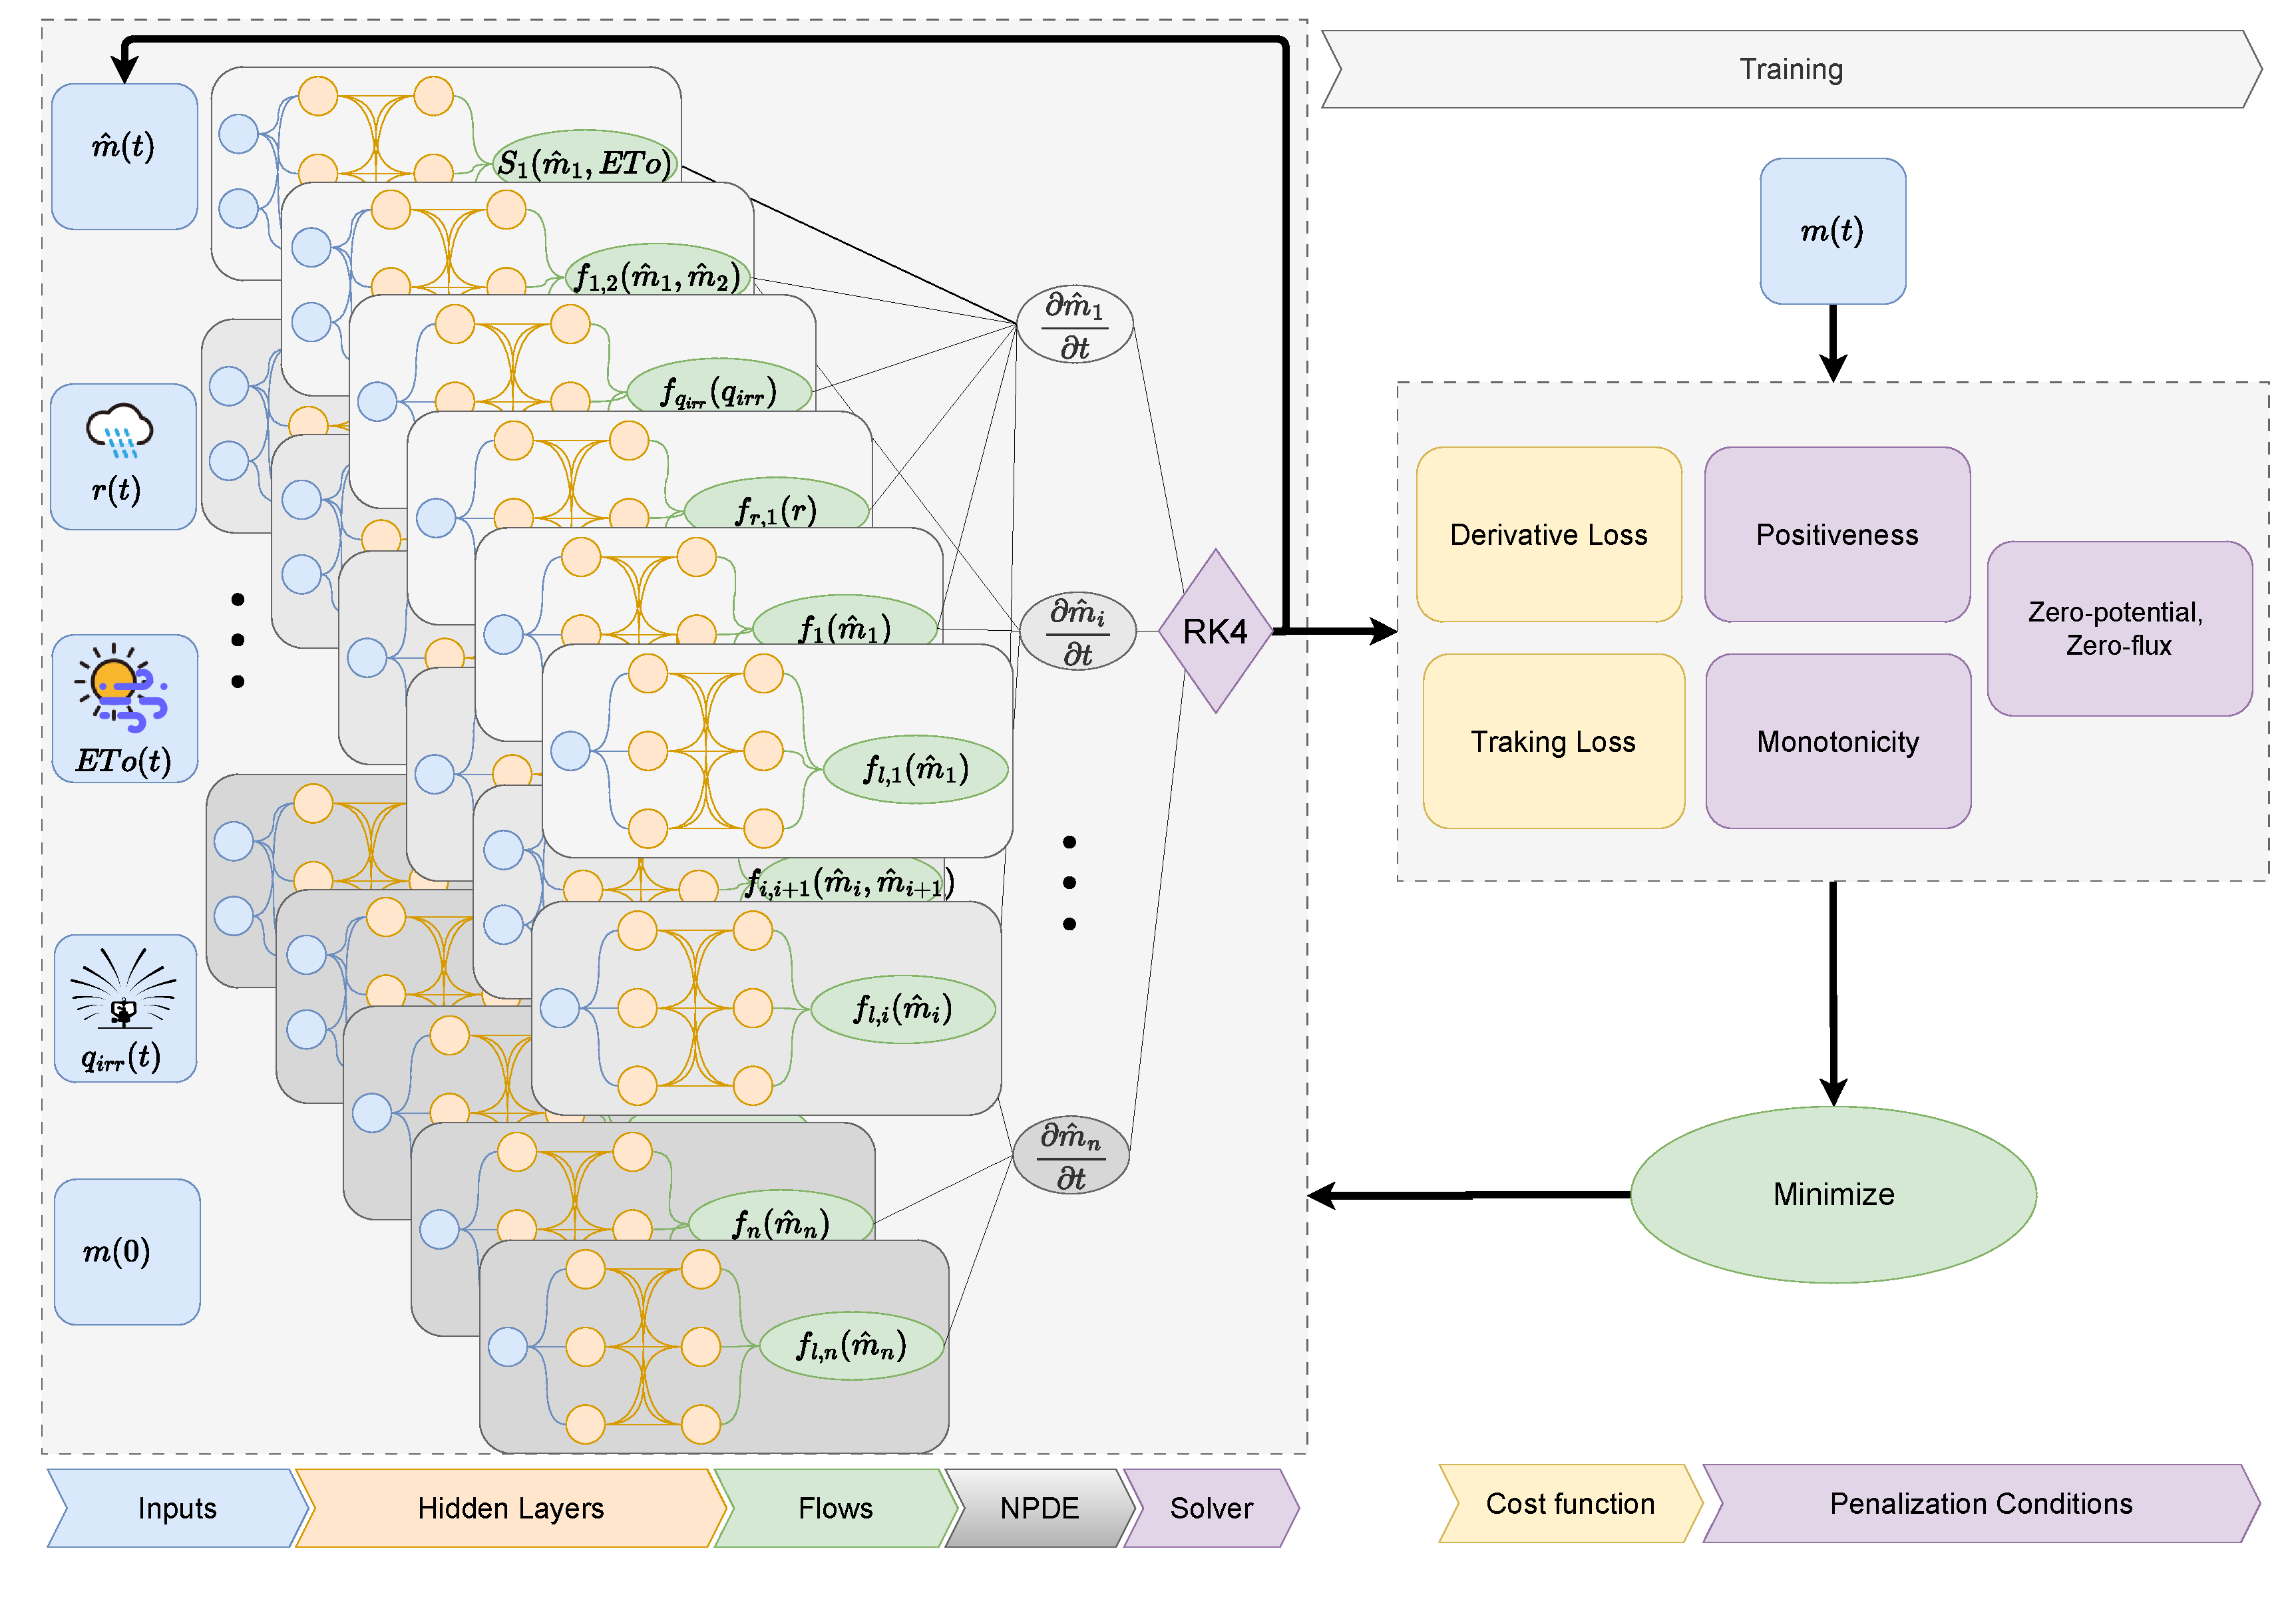
\includegraphics[width=0.8\textwidth]{PINNsmb.pdf}
		\caption{Schematic for the description of the proposed PINN related to data available in a real system}
		\label{diagramalgorithm}
  \vspace{-1em}
\end{figure}

\subsubsection{Model}\label{sec2}

The developed Physics-Informed Neural Network (PINN) is formulated using a spatial discretization of Richards' equation, which describes vertical water movement in the soil as a function of soil moisture. We propose a spatial discretization by dividing the soil into $n$ layers, with each layer associated with available soil moisture measurements. The objective is to determine the rate of change of soil moisture in each layer due to gravity and water potential. In porous media, the Richards' equation is classically expressed as:

\begin{equation}
\frac{\partial m}{\partial t} = \frac{\partial }{\partial z}\left[ K(m)\left(\frac{\partial h(m)}{\partial z}+1\right)\right]
\label{Richards}
\end{equation}
Where $m$ is the soil moisture, $z$ is the vertical axis, considered to increase downward, $K(m)$ is the hydraulic conductivity, which depends on soil moisture, and $h(m)$ is the soil-water pressure head.

The Richards' equation obeys the continuity relation; thus, by defining $q$ as a water flux, the continuity relation is given by:
\begin{equation}
\frac{\partial m}{\partial t} = -\frac{\partial q}{\partial z}
\label{continuity}
\end{equation}

Therefore, from Eq.\ref{Richards} and Eq. \ref{continuity} , the Darcy-Buckingham law can be extracted as:
\begin{equation}
q = K(m)\left(\frac{\partial h(m)}{\partial z}+1\right)
\end{equation}
If a spatial discretization along $z$ with a fixed spatial step $\Delta z$ is proposed, the flux $q_i$ leaving layer $i$ downwards to the layer $i+1$ is given by:
\begin{equation}
q_i = K(m_i)\left(\frac{h(m_i)-h(m_{i+1})}{\Delta z}+1\right)
\end{equation}
Similarly, the continuity equation describing moisture conservation in a layer $i$ can be discretized as:
\begin{equation}
\frac{d m_i}{d t} = \frac{q_{i-1}(t)-q_i(t)}{\Delta z}.
\end{equation}

Therefore, a discretized description of soil water dynamics at a layer $i$ is provided by

\begin{equation}
\frac{d m_i}{d t} = K(m_{i-1})\left(\frac{h(m_{i-1})-h(m_{i})}{\Delta z^2}\right) + \frac{K(m_{i-1})}{\Delta z} - K(m_{i})\left(\frac{h(m_{i})-h(m_{i+1})}{\Delta z^2}\right) - \frac{K(m_{i})}{\Delta z}.
\end{equation}


From this discretized formulation, it can be observed that the rate of change of soil moisture at each i-th layer, driven by gravity and potential forces, can be described as functions (to be estimated) of measured soil moisture in the respective and adjacent layers. Specifically, we are proposing a structure where

\begin{equation}
\begin{aligned}
K(m_{i})\left(\frac{h(m_{i})-h(m_{i+1})}{\Delta z^2}\right) &\approx f_{i,i+1}({m}_i,{m}_{i+1}), \\ 
\frac{K(m_{i})}{\Delta z} &\approx f_i({m}_i).
\end{aligned}
\end{equation}



Moreover, additional functions describing the rate of change produced by actions such as irrigation, rainfall, water uptake, and horizontal water movement can be incorporated to obtain a model structure that could be useful for evaluating how soil moisture dynamics evolve over time in response to external variables. In specific, $q_{irr}$ is incorporated as the irrigation related variable, and $fq_{irr}(q_{irr})$ is a function that explains the rate of change of the soil moisture in relation to irrigation, note that $q_{irr}$ could have units of flow (e.g., \si{m3/h}) or units of relative time (e.g., \si{h/h}) indicating how much irrigation was active during a period of time. In the first case, $fq_{irr}(q_{irr})$ provides a relation between applied flow and change in soil moisture, and in the second case, $fq_{irr}(q_{irr})$  provides a relation between duration of irrigation time and change in soil moisture. In this study, we assume that irrigation is applied only at the top, but its location can be accommodated depending on the irrigation system used, e.g., subsurface drip irrigation. 
The rainfall, $r$, is considered an input in \si{mm/h} and can be obtained from a weather station in the crop or from meteorological services, where predictions are also available. The function, $fr_i(r)$, accounts for the direct effect of rain at each soil layer. This is because crops are often planted in beds, allowing rain to wet exposed soil layers directly.

Furthermore, we incorporate a sink component to estimate soil moisture changes due to plant uptake in each layer, which is a key motivation for this study. This sink is represented by a plant coefficient, $S_i (m_i, ET_0)$, describing plant uptake at each layer. This uptake is determined by atmospheric, plant, and soil conditions \cite{swap2024}. Specifically, we propose that this uptake is a function of the available water at the respective layer ($m_i$) and the potential evapotranspiration ($ET_0$).

Additionally, we include an outlet lateral flow, $fl_i (m)$, associated with runoff when excess water prevents flow between layers. This is considered an outlet, as most crops are planted in raised beds between furrows to facilitate drainage.

In summary, we are formulating a PINN to estimate the dynamics of a system with $n$ soil layers as follows:

\begin{equation}
\label{system}
\begin{aligned}
\frac{d{m}_1}{dt} = & - f_1({m}_1) - f_{1,2}({m}_1,{m}_2) - fl_1 (m_1) - S_1({m}_1, ET_0) + fr_1(r) + fq_{irr}(q_{irr})\\
\frac{d{m}_i}{dt} = & f_{i-1}({m}_{i-1}) + f_{i-1,i}({m}_{i-1},{m}_i) - f_i({m}_i)- f_{i,i+1}({m}_i,{m}_{i+1}) - fl_i (m) - . . .\\ 
 & S_i({m}_i, ETo) + fr_i(r), \\
\frac{d{m}_n}{dt} = & f_{n-1}({m}_{n-1}) + f_{n-1,n}({m}_{n-1},{m}_n) - f_n({m}_n)    - S_n({m}_n, ETo) + fr_n(r),
\end{aligned}
\end{equation}
Note that at layer $n$, we exclude the lateral flow term $fl_n$. In the upper layers, the vertical flow $f_i$ delivers water to the layer below, making it distinct from the lateral flow $fl_i$, which exits the system. However, at layer $n$, both $f_n$ and $fl_n$ would represent outflows that leave the soil column without feeding another layer, making them similar.

\subsubsection{PINN Structure}
In our approach, we use the system structure proposed in (Eq. \eqref{system}) to define the PINN structure. Therefore, as shown in Fig. \ref{diagramalgorithm}, we are proposing an NN with branches that emulate the functions \( g \in \{f_i, f_{i,i+1}, S_i, fq_{irr}, fr_i,fl_i\} \). Therefore, each branch is a Multilayer Perceptron (MLP) with depth \( L \) and width \( H \), given by
\begin{equation}
\phi\!\bigl(\mathbf{x}; \boldsymbol{\Theta}\bigr)
  =\;
  \mathbf{W}^{(L)}
  \,\mathcal{A}\!\Bigl(
     \mathbf{W}^{(L-1)}
     \,\mathcal{A}\!\bigl(
        \dots
        \,\mathcal{A}\!\bigl(
           \mathbf{W}^{(1)}\mathbf{x}
           +\mathbf{b}^{(1)}
        \bigr)
        +\mathbf{b}^{(L-1)}
     \bigr)
  \Bigr)
  +\mathbf{b}^{(L)},
\label{eq:mlp}
\end{equation}


where \(\mathcal{A}(\cdot)\) is the activation function, and  
\(\displaystyle \boldsymbol{\Theta} = \{\mathbf{W}^{(\ell)},\,\mathbf{b}^{(\ell)}\}_{\ell=1}^L\) is the set of trainable parameters. The input \(\mathbf{x}\) denotes the argument of each flux function.  
In cases where the function depends on a single variable $\left(f_i(m_i),\;f_q(q),\;f_{r_i}(r),\;f_{l_i}(m)\right)$, we have \(\mathbf{x}\in\mathbb{R}\), and when the function depends on two variables \(f_{i,i+1}(m_i,m_{i+1})\),  
\(\displaystyle \mathbf{x}=[m_i,m_{i+1}]\in\mathbb{R}^2\); and for \(S_i(m_i,\mathrm{ET_0})\),  
\(\displaystyle \mathbf{x}=[m_i,\mathrm{ET_0}]\in\mathbb{R}^2\).  Moreover, the dimensions of the first-layer weight matrices are  
\(\mathbf{W}^{(1)}\in\mathbb{R}^{H\times1}\) for scalar inputs, and  
\(\mathbf{W}^{(1)}\in\mathbb{R}^{H\times2}\) for two-dimensional inputs as encountered in \(f_{i,i+1}\) and \(S_i\).
\( \mathbf{W}^{(\ell)} \in \mathbb{R}^{H \times H} \) for \( \ell = 2, \dots, L-1 \), and \( \mathbf{W}^{(L)} \in \mathbb{R}^{1 \times H} \). With biases \( \mathbf{b}^{(\ell)} \in \mathbb{R}^{H} \) for \( \ell = 1, \dots, L-1 \), and \( \mathbf{b}^{(L)} \in \mathbb{R} \).

Note that for brevity, a compact description of the system can be formulated as 

\begin{equation}
    \label{systemtheta}
    \dot{m}(t) = g(m,r,ET_0,q,\boldsymbol{\Theta})
\end{equation}


\subsubsection{Optimization Problem and Training}\label{subsec2}

As shown in the model formulation, PINN is a highly flexible technique that allows incorporating all physical and even empirical knowledge about the system into the PINN structure. Additionally, the formulation of the optimization problem provides an opportunity to shape the estimated system, including information that can contribute to model generalization and the estimated system's physical correctness. Therefore, the optimization problem is formulated to parameterize the system \ref{systemtheta}, aiming that this: i) mimics soil-water and plant water uptake dynamics; ii) provides a clear explanation of the effects of the considered fluxes on the system; and ii) is useful for the design of control or decision-making approaches, especially predictive control approaches.

\subsubsection{Data Preparation for Training}

The approach uses a moving-horizon data window for training, enabling a model that can be periodically tuned using stored system measurements, consistent with the strategy presented in \cite{condeforecast2024}. To simplify neural network training and avoid extensive normalization analysis, all input data (e.g., soil moisture, irrigation, rainfall, and evapotranspiration) are assumed to be normalized to the range [0, 1]. To clarify the estimation process, the following notation is introduced, where \( n_e \) is the size of the estimation window and \( t_k \) is the current time instant.

Let \( m(t_k) = [m_1(t_k), m_2(t_k), \dots\ m_n(t_k)] \in \mathbb{R}^{n} \) denote the measured soil moisture at $n$ depths at the current time \( t_k \), and 

let \( m_i(t_{k_e \mid k}) \) the time series of measurements at depth \( i \) over an estimation window of size $n_e$, defined as  
${m_i(t_{k_e \mid k})}=\left[m_i(t_{k-n_e +1}), m_i(t_{k-n_e +2}), ...\ m_i(t_{k}) \right]^\top \in \mathbb{R}^{n_e}$;


Then, the full set of measured soil moisture data over the estimation window is given by 
\[
m(t_{k_e \mid k}) = \begin{bmatrix}
m_1(t_{k_e \mid k}) & m_2(t_{k_e \mid k}) & \cdots & m_n(t_{k_e \mid k})
\end{bmatrix} \in \mathbb{R}^{n_e \times n}. 
\] 

Therefore, along the same estimation window, the set of estimated soil moisture is given by  

\[
\hat{m}(t_{k_e \mid k}) = \begin{bmatrix}
\hat{m}_1(t_{k_e \mid k}) & \hat{m}_2(t_{k_e \mid k}) & \cdots & \hat{m}_n(t_{k_e \mid k})
\end{bmatrix} \in \mathbb{R}^{n_e \times n}, 
\] 
where $\hat{m}$ is introduced to differentiate estimated soil moisture from measured soil moisture $m$. 

Similarly, it is defined $\Delta m(t_k) \in \mathbb{R}^{n}$ as 
\[
\Delta m(t_k) = m(t_k)-m(t_k-1),
\]
and $\Delta \hat{m}(t_k) \in \mathbb{R}^{n} $ as 

\[
\Delta \hat{m}(t_k) = g(m(t_k),r(t_k),ET_0 (t_k),q(t_k),\boldsymbol{\Theta}(t_k)),
\]


The measured rain, irrigation, and computed potential evapotranspiration along the estimation process are defined as 
${r(t_{k_e \mid k})}=\left[r(t_{k-n_e +1}) \ r(t_{k-n_e +2}) \ ...\ r(t_{k}) \right]^\top \in \mathbb{R}^{n_e}$, 
${q(t_{k_e \mid k})}=\left[q(t_{k-n_e +1}) \ q(t_{k-n_e +2}) \ ...\ q(t_{k}) \right]^\top \in \mathbb{R}^{n_e}$,
and 
${Et_0 (t_{k_e \mid k})}=\left[Eto (t_{k-n_e +1}) \ Eto (t_{k-n_e +2}) \ ...\ Eto (t_{k}) \right]^\top \in \mathbb{R}^{n_e}$, 
respectively. 

Based on the available data, we aim to formulate an optimization problem to minimize the error between measured and estimated soil moisture while addressing physical constraints.

\subsubsection{Estimation Approach}
Our goal is to estimate the parameters $\boldsymbol{\Theta}$ of the system 
\begin{equation}
    \dot{\hat{m}}(t) = g(\hat{m},r,ET_0,q,\boldsymbol{\Theta}),
\end{equation}
with initial conditions \(\hat{m}(t_{k-n_e+1}) = m(t_{k-n_e+1})\), and solution over the window \(t\in[t_{k-n_e+1},\,t_k]\) given by

\begin{equation}
\label{integral}
    \hat{m}(t_k)
  \;=\;
  m(t_{k-n_e+1})\;+\;
  \int_{t_{k-n_e+1}}^{t}
        g\!\bigl(
            \hat{m}(\tau),
            r(\tau),
            \mathrm{ET_0}(\tau),
            q(\tau),
            \boldsymbol{\Theta}
          \bigr)\, d\tau,
  \quad t\in[t_{k-n_e+1},t_k].
\end{equation}
The state trajectory $ \hat{m}(t_{k - n_e + 1 \mid k}) $ is obtained from $ \hat{m}(t_k) $ at discrete time points $ t_{k - n_e + 1}, \dots, t_k $. In practice, the integral in \eqref{integral} is approximated using numerical strategies such as direct multiple shooting, direct collocation, or successive linearizations. A simpler alternative, such as the Euler discretization, is less accurate and is therefore not considered here. We propose a direct multiple-shooting method that employs an RK4 method with a lower bound to prevent negative solutions for the estimated soil moisture. This method is selected for its widespread use and high accuracy in solving ordinary differential equations (ODEs) \cite{rawlings2017}. 

The inclusion of numerical integration of the system dynamics in the cost function is common in model-based approaches, such as moving horizon estimation (MHE) \cite{rawlings2017}. This inclusion contributes to the generality and stability of the estimated model, since the estimated parameters must induce a trajectory that replicates the real system’s evolution, making the model more robust to data variations and potentially better suited for generalization to unseen scenarios. Moreover, during optimization, unstable solutions yield large estimation errors, thereby guiding the solution toward parameters that promote the system's stability. 

However, as mentioned, directly incorporating the numerical integration of system dynamics into the cost function complicates the optimization problem, hindering the optimizer's ability to identify suitable solutions. To address this, the training process is divided into two stages.


In the first stage, the cost function is formulated by formulating a typical weighted mean square error defined as:
\begin{equation}
    j_{1}(\boldsymbol{\Theta}) = 
    \frac{1}{n_e} \sum_{t_k = t_{k - n_e + 1}}^{t_k} 
    \left\| 
         \left( 
            \Delta m(t_k) - g(m(t_k), r(t_k), \mathrm{ET_0}(t_k), q(t_k), \boldsymbol{\Theta}) 
        \right) 
    \right\|_{\mathbf{W}_1}^2,
    \label{eq:j1}
\end{equation}
where \( \Delta m(t_k) = m(t_k) - m(t_{k-1}) \) represents the change in soil moisture between consecutive time steps, and \( t_k \) denotes the current time with the summation over the estimation window \( [t_{k - n_e + 1}, t_k] \). The weight matrix \( \mathbf{W}_1 = \operatorname{diag}(\sigma_{1,\Delta}^{-1}, \dots, \sigma_{n,\Delta}^{-1}) \) balances the influence of different soil layers, with variances computed as:
\[
    \sigma_{i,\Delta}^{2} = \frac{1}{N} \sum_{k=1}^{N} \left( \Delta m_i(t_k) - \overline{\Delta m_i} \right)^{2},
\]
where \( \overline{\Delta m_i} = \frac{1}{N} \sum_{k=1}^{N} \Delta m_i(t_k) \) is the mean of \( \Delta m_i(t_k) \) over a dataset of size \( N \).

This stage aims to obtain an initial estimate of \( \boldsymbol{\Theta} \) that approximates the rate of change of soil moisture, providing a starting point for subsequent refinement.

In the second stage, we opted to formulate the cost function using a weighted mean absolute error to balance the high soil moisture increases caused by rain and irrigation with the small soil moisture decreases caused by evapotranspiration, as follows:
\begin{equation}
    j_{2}(\boldsymbol{\Theta}) = 
    \frac{1}{n_e} \sum_{t_k = t_{k - n_e + 1}}^{t_k} 
    \left\| 
         \left( 
            m(t_k) - \hat{m}(t_k) 
        \right) 
    \right\|_{\mathbf{W}_2},
    \label{eq:j2}
\end{equation}
where \( \hat{m}(t_k) \) is the soil moisture trajectory obtained from numerically integrating the system dynamics, as described in \eqref{integral}. 

Similarly, it is included a weight matrix \( \mathbf{W}_2 = \operatorname{diag}(\sigma_{1,m}^{-1}, \dots, \sigma_{n,m}^{-1}) \) with variances:
\[
    \sigma_{i,m}^{2} = \frac{1}{N} \sum_{k=1}^{N} \left( m_i(t_k) - \overline{m_i} \right)^{2},
\]
and  \( \overline{m_i} = \frac{1}{N} \sum_{k=1}^{N} m_i(t_k) \).


%%%%



\subsubsection{Penalizations}
To enforce the estimated flux functions adhere to principles such as non-negativity, monotonicity, and zero-flow conditions, we define three penalization terms, \( c_1 \), \( c_2 \), and \( c_3 \). These terms are evaluated using synthetic data with \( M = 1000 \) random samples to evaluate the entire space of each flux function. This approach ensures that the constraints hold globally, across all possible operating conditions, rather than being limited to the measured dataset.

\textbf{Penalization Term \( c_1 \): Non-Negativity Constraint}
The term \( c_1 \) ensures the non-negativity of flux functions, thereby ensuring physical consistency in processes such as infiltration, drainage, and evapotranspiration by preventing negative fluxes that would violate mass balance. It is defined as:
\[
c_1 = \lambda_{c_1} \frac{1}{M} \sum_{k=1}^M \sum_{g \in \mathcal{G}} \left( \min(0, g(\mathbf{x}_k)) \right)^2,
\]
where \( \mathcal{G} = \{ f_1, \dots, f_{n-1}, f_{1,2}, \dots, f_{n-1,n}, fq, fr_1, \dots, fr_n, S_1, \dots, S_n, fl_1, \dots, fl_{n-1} \} \) denotes the set of flux functions, \( g(\mathbf{x}_k) \) is the flux evaluated at random samples \( \mathbf{x}_k \) from its input space (e.g., \( \mathbf{x}_k = m_{i,k} \) for \( g = f_i(m_i) \), or \( \mathbf{x}_k = [m_{i,k}, m_{i+1,k}] \) for \( g = f_{i,i+1}(m_i, m_{i+1}) \)), and \( M = 1000 \) is the number of samples. Note that \( f_n \) is excluded, as their flow direction at the boundary depends on external conditions.

\textbf{Penalization Term \( c_2 \): Monotonicity Constraint}
The term \( c_2 \) ensures that flux functions increase (or remain constant) with their driving variables, reflecting the physical expectation that fluxes should not decrease with higher moisture, irrigation, rainfall, or evapotranspiration demand. It is given by:
\[
c_2 = \lambda_{c_2} \frac{1}{M} \sum_{k=1}^M \sum_{d \in \mathcal{D}} \left( \min(0, d(\mathbf{x}_k)) \right)^2,
\]
where \( \mathcal{D} = \{ \frac{\partial fq}{\partial q}, \frac{\partial fr_1}{\partial r}, \dots, \frac{\partial fr_n}{\partial r}, \frac{\partial f_1}{\partial m_1}, \dots, \frac{\partial f_{n-1}}{\partial m_{n-1}}, \frac{\partial f_{1,2}}{\partial (m_1 - m_2)}, \dots, \frac{\partial f_{n-1,n}}{\partial (m_{n-1} - m_n)}, \frac{\partial S_1}{\partial m_1}, \\ 
\dots, \frac{\partial S_n}{\partial m_n}, \frac{\partial S_1}{\partial ET_0}, \dots, \frac{\partial S_n}{\partial \text{ETo}}, \frac{\partial fl_1}{\partial m_1}, \dots, \frac{\partial fl_{n-1}}{\partial m_{n-1}} \} \) is the set of partial derivatives, evaluated at random samples \( \mathbf{x}_k \) (e.g., \( \mathbf{x}_k = m_{i,k} \) for \( d = \frac{\partial f_i}{\partial m_i} \)). Monotonicity is not enforced for \( f_n \) due to potential non-monotonic behavior at the boundary.

\textbf{Penalization Term \( c_3 \): Zero-Flow Condition}
The term \( c_3 \) ensures that flux functions, such as drainage or irrigation, are zero when their driving variables (e.g., soil moisture or irrigation rate) are zero or nearly zero, as no flow should occur without a driving force. It is defined as:
\[
c_3 = \lambda_{c_3} \frac{1}{M} \sum_{k=1}^M \sum_{g \in \mathcal{G}_0} g(\mathbf{x}_k)^2 \cdot \delta_k,
\]
where \( \mathcal{G}_0 = \{ f_1, \dots, f_{n-1}, f_{1,2}, \dots, f_{n-1,n}, fq, fr_1, \dots, fr_n, S_1, \dots, S_n, fl_1, \dots, fl_{n-1} \} \), \( g(\mathbf{x}_k) \) is the flux evaluated at random samples across its input space, and \( \delta_k = 1 \) if the driving variable (e.g., soil moisture for \( f_i \), or both soil moisture and \( ET_0 \) for \( S_i \)) is smaller than \( \epsilon = 10^{-7} \), and \( \delta_k = 0 \) otherwise. \( f_n \) is also excluded in this constraint.

At the end, we have $\lambda_{c_1}$, $\lambda_{c_2}$, and $\lambda_{c_3}$ and also the number of layers $L$, and number of neurons per layer $H$ as hyper parameters to be selected. In our algorithm, we are using $L=4$ for functions that depend on one input variable, such as $f_i, fq, fr_i,$ and $fl_i$; and $L=5$ for functions that depend on two variables, such as $S_i$, and $f_{i, i+1}$. Respecting $\lambda_{c_1}$, $\lambda_{c_2}$, $\lambda_{c_3}$, and $H$ we are utilizing an hyperparametrization tool. 


\subsection{Case Study} \label{Test Case}
The proposed approach has been tested using field data from the Millennium Block at the Indian River Research and Education Center (IRREC) in Fort Pierce, Florida. This 35-acre citrus trial site is dedicated to exploring multiple breeding lines for tolerance to Huanglongbing (HLB; greening). Actively, 20 acres host a 6-year-old experiment evaluating grapefruit, grapefruit-like, sweet orange, and mandarin varieties from the University of Florida and USDA programs, grafted onto distinct rootstocks, comprising 5,500 trees across four trials. The site's Classical Alfisols are poorly drained, with a shallow sandy profile over clay that limits root growth to ~30 cm, a condition exacerbated by seawater intrusion. Trees are planted on raised beds surrounded by ditches to mitigate salinity, promote drainage, and support shallow citrus roots. Irrigation uses sprinklers every other day for 2 hours in summer (sourced from an onsite well, skipped post-precipitation), with 90-day slow-release 10-2-12 fertilizer at 3.5 lb/tree, foliar micronutrients 4x/year, and pest/disease control as identified.

\begin{figure}
\centering
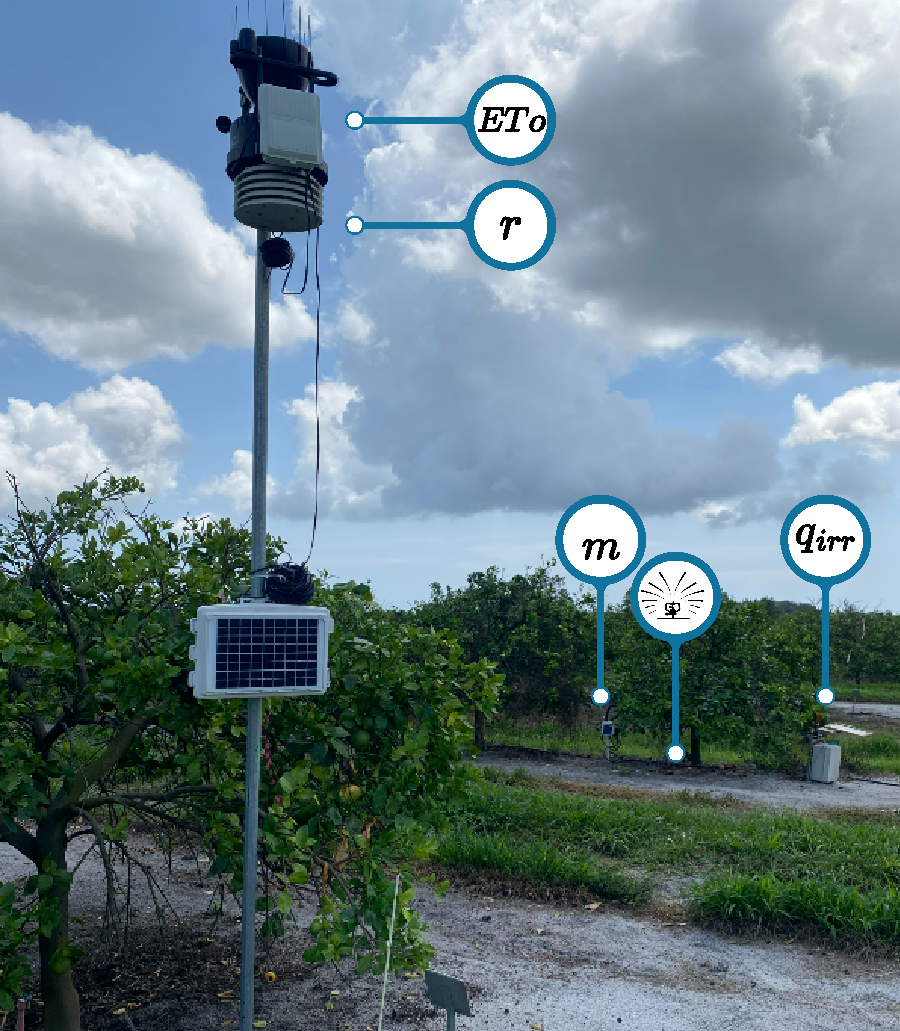
\includegraphics[width=0.5\linewidth]{sensorsmillenniumb.pdf}
\caption{Description of experimental setup, where a weather station, soil moisture probe, and irrigation sensor were deployed to collect soil moisture ($m$), rain ($r$), potential evapotranspiration ($ET_0$), and irrigation ($qirr$) data.}
\label{sensorsmillennium}
\end{figure}

In a designated section of the Millennium Block, multiple sensors were installed (Fig. \ref{sensorsmillennium}), with data collected, processed, and stored using Irrigmonitor, a custom cloud-based application that facilitates real-time data integration for agricultural water management. The following instrumentation was deployed:
\begin{description}
\item[Weather Station:] A Davis Vantage Pro2 weather station\footnote{See \url{https://www.davisinstruments.com/pages/vantage-pro2} for more information on Davis weather stations.} providing rainfall and meteorological variables (temperature, humidity, wind speed, solar radiation, and barometric pressure). These data were employed to calculate $ET_0$ using the Penman-Monteith method \cite{allen1998crop}.
\item[Soil Moisture Probe:] SM measurements were taken at 5\si{cm}, 15\si{cm}, 25\si{cm}, 35\si{cm}, 45\si{cm}, 55\si{cm} using a Sentek Drill \& Drop probe\footnote{Series II Sentek Drill \& Drop probe, capable of measuring SM, temperature, and salinity at 10\si{cm} intervals. See \url{https://sentektechnologies.com/download/sentek-drill-drop-probe-manual/} for details.}, located 20\si{cm} from the base of the tree.
\item[Irrigation Sensor:] Irrigation events were detected by installing two electrodes at the supply irrigation point, connected to a Campbell Scientific CR1000X datalogger, where changes in electrical conduction were used to identify irrigation events and their duration (\si{h/h}).
\end{description}

We collected 864 hours (36 days) of data from March 28, 2025, 20:00:00 to May 2, 2025, 20:00:00, for training. This period included approximately seven distinct rain events (Fig. \ref{Mainfig}). The duration of the training window was selected to ensure a sufficient number of rain events, which are scarce compared to other variables, such as reference evapotranspiration, which changes continuously, or irrigation events, which can be controlled to generate data. Further research on optimizing the estimation window duration and addressing scenarios with limited rainfall is planned, but is beyond the scope of this study.
Additionally, we collected 72 hours (3 days) of data from May 3, 2025, 21:00:00 to May 6, 2025, 21:00:00, for validation. This 3-day validation window aligns with the typical 3-day prediction horizon of weather forecast data from sources such as the National Weather Service \cite{NWS2024}, which can be integrated into the algorithm for predictive irrigation management. This duration assesses the approach's effectiveness in leveraging short-term weather forecasts for irrigation scheduling.
All data were processed and standardized to a one-hour sampling interval to match the temporal resolution of weather forecast data \cite{NWS2024}. This sampling interval was chosen as a constraint because although sensors can collect data at smaller temporal scales, irrigation management strategies that integrate weather forecasts must rely on the temporal resolution of available forecast data.
\subsection{Computational Tools and Algorithm Setup}
The PINN was implemented using TensorFlow 2.10, with 64-bit floating-point precision (\texttt{float64}) to promote numerical stability and accuracy. TensorFlow’s automatic differentiation (synthetic differentiation) was employed to compute gradients and embed physical constraints directly into the training process.
The numerical integration of the PINN’s differential equations was performed using a custom RK4 solver fully integrated into TensorFlow’s computational graph.

% Source code: FINAL_SUBMISSION/code/pinn_training.py (derived from Pinparameb.py)
% Figures: FINAL_SUBMISSION/code/paper_figures.ipynb
% Optuna: optuna_stage1b.py (Stage 1, 200 trials), PINN_optuna_stage2.py (Stage 2, 30 trials)
Hyperparameter optimization was performed using Optuna 3.5, a Bayesian optimization framework, across 200 trials for Stage 1, each evaluated for 150 epochs using the derivative loss ($j_1$), followed by 30 trials for Stage 2. Key hyperparameters obtained included:
\begin{itemize}
\item Initial learning rate for Stage 1 ($\eta_1$): \num{7.97e-5}.
\item Number of neurons per layer ($H$): 56.
\item Loss weight multipliers: $\lambda_{c_1} = \num{113982766}$, $\lambda_{c_2} = \num{1773295}$, and $\lambda_{c_3} = \num{126704656}$.
\end{itemize} 

\section*{Funding}
This research was supported by the United States - Israel Binational Agricultural Research and Development Fund (Grant ID IS-5774-25) and the Florida Department of Agriculture and Consumer Services (Grant ID 33200).

\section*{Data availability}
The datasets generated and/or analyzed during the current study, along with the inference code, are available in the Zenodo repository, https://doi.org/10.5281/zenodo.19446129. The custom training code used to develop the Physics-Informed Neural Network is proprietary and not publicly available, but is available to editors and reviewers upon request for manuscript evaluation.

\bibliography{PINN}% common bib file


\end{document}